% leastUPO.tex
%
% Predrag created file              Apr 12 2007
% $Author$ $Date$


%%%%%%%%%%%%%%%%%%%%%%%%%%%%%%%%%%%%%%%%%%%%%%%%%%%%%%%%%%%%%%%%
\begin{figure}[t]
\begin{center}
(a) 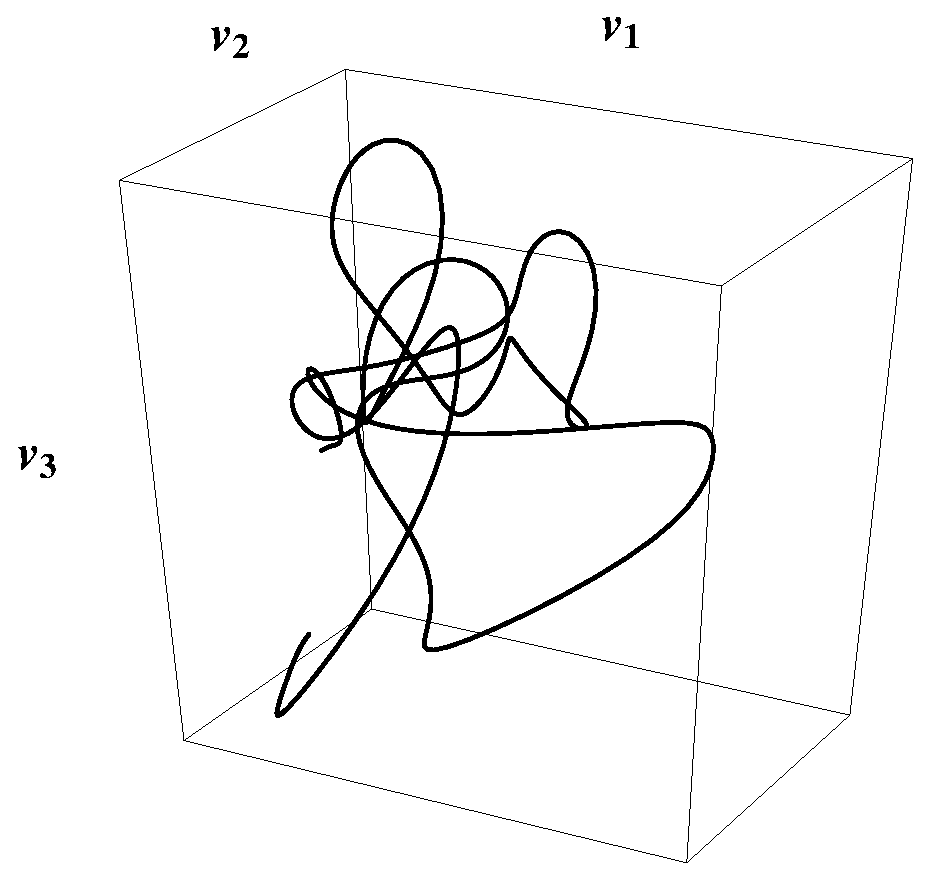
\includegraphics[width=0.35\textwidth]{figs/ks22rpo033.50_04.045E2.eps}
(b) 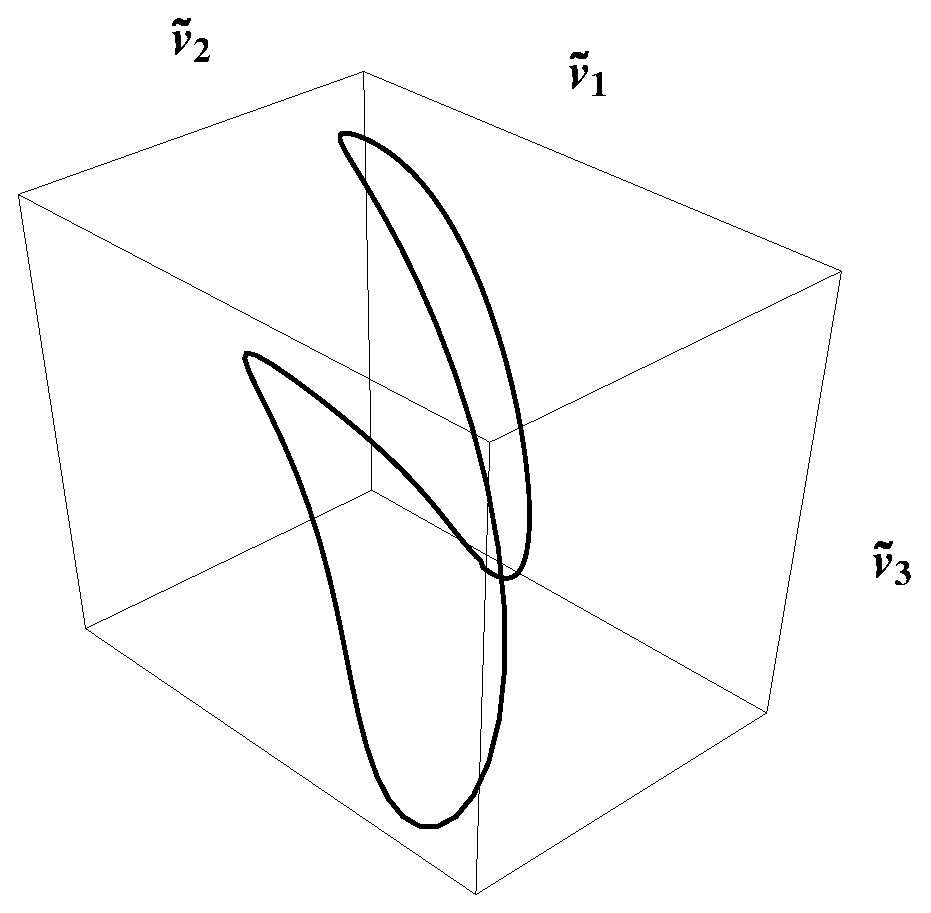
\includegraphics[width=0.35\textwidth]{figs/ks22rpo033.50_04.045E2CM.eps}
\\
\end{center}
\caption{
 The
which appears well embedded within the turbulent flow. 
\rpo\ with $(\period{p},\shift_p) =(33.5,4.04)$
from \reffig{f:ks22rposShort}\,(\textit{c}) in:
 (a) \Statesp, traced for four periods $\period{p}$. The coordinate axes
$v_1$, $v_2$, and $v_3$ are those of \reffig{f:KS22E2man}.
 (b) Mean velocity frame.
        } \label{f:MeanVelocityFrame}
\end{figure}
%%%%%%%%%%%%%%%%%%%%%%%%%%%%%%%%%%%%%%%%%%%%%%%%%%%%%%%%%%%%%%%%%%



Sets of \rpo s are difficult to visualize simultaneously.
Somewhat better visualization is in the
{\em mean velocity frame}, {\ie},
a reference frame that rotates with with velocity
$v_p=\shift_p/\period{p}$.
In the mean velocity frame a \rpo\ becomes
a \po, see  for example \reffig{f:MeanVelocityFrame}.
On the other hand each {\rpo} has its own mean velocity frame and thus
the simultaneous visualization of \rpo s becomes problematic.

As the shift $d$ is defined mod~$L$, better to
state for each {\rpo} its mean velocity $c_p = \shift_p/\period{p}$,
where $\shift_p$ is measured on the line (not on the circle). $c_p$ is
preferable to angle $2\pi \shift_p/L$ as it does not vary in $L \to$~large
limit (just like $\sqrt{2}$ wavelength estimate is independent of
system size).
